%% ============================================================
%%  CSIR-UGC NET Mathematical Sciences — Preparation Blueprint
%%  Based on December 2025 & June 2025 Question Papers
%%  Compile with: pdflatex (twice for TOC)
%% ============================================================
\documentclass[12pt,a4paper]{article}

%% --- Packages ---
\usepackage[a4paper, top=2.2cm, bottom=2.2cm, left=2.5cm, right=2.5cm]{geometry}
\usepackage{amsmath,amssymb}
\usepackage{xcolor}
\usepackage{array}
\usepackage{booktabs}
\usepackage{longtable}
\usepackage{multirow}
\usepackage{enumitem}
\usepackage{mdframed}
\usepackage{tikz}
\usepackage{pgfplots}
\pgfplotsset{compat=1.18}
\usepackage{tcolorbox}
\tcbuselibrary{skins,breakable,most}
\usepackage{fontenc}
\usepackage{inputenc}


\usepackage{fancyhdr}
\setlength{\headheight}{15pt}
\usepackage{titlesec}
\usepackage{hyperref}
\usepackage{graphicx}
\usepackage{wrapfig}
\usepackage{tabularx}
\usepackage{colortbl}
\usepackage{makecell}
\usepackage{parskip}
\usepackage{setspace}


%% --- Hyperref setup ---
\hypersetup{
  colorlinks=true,
  linkcolor=blueprimary,
  urlcolor=blueprimary,
  pdftitle={CSIR NET Maths Blueprint},
  pdfauthor={Blueprint Generator},
  pdfsubject={CSIR-UGC NET Mathematical Sciences Preparation}
}

%% ============================================================
%%  COLOR PALETTE
%% ============================================================
\definecolor{blueprimary}{RGB}{24,95,165}
\definecolor{bluelight}{RGB}{230,241,251}
\definecolor{bluedark}{RGB}{12,68,124}
\definecolor{redprimary}{RGB}{226,75,74}
\definecolor{redlight}{RGB}{252,235,235}
\definecolor{reddark}{RGB}{121,31,31}
\definecolor{purpleprimary}{RGB}{83,74,183}
\definecolor{purplelight}{RGB}{238,237,254}
\definecolor{purpledark}{RGB}{60,52,137}
\definecolor{amberprimary}{RGB}{239,159,39}
\definecolor{amberlight}{RGB}{250,238,218}
\definecolor{amberdark}{RGB}{99,56,6}
\definecolor{greenprimary}{RGB}{99,153,34}
\definecolor{greenlight}{RGB}{234,243,222}
\definecolor{greendark}{RGB}{39,80,10}
\definecolor{tealprimary}{RGB}{29,158,117}
\definecolor{teallight}{RGB}{225,245,238}
\definecolor{tealdark}{RGB}{8,80,65}
\definecolor{grayprimary}{RGB}{136,135,128}
\definecolor{graylight}{RGB}{241,239,232}
\definecolor{graydark}{RGB}{68,68,65}
\definecolor{coralight}{RGB}{250,236,231}
\definecolor{coradark}{RGB}{113,43,19}
\definecolor{bgpage}{RGB}{252,252,250}
\definecolor{bgsection}{RGB}{245,245,242}

%% ============================================================
%%  PAGE STYLE
%% ============================================================
\pagestyle{fancy}
\fancyhf{}
\fancyhead[L]{\small\color{grayprimary}\textbf{CSIR-UGC NET} Mathematical Sciences — Preparation Blueprint}
\fancyhead[R]{\small\color{grayprimary}Dec 2025 \& Jun 2025 Analysis}
\fancyfoot[C]{\small\color{grayprimary}\thepage}
\renewcommand{\headrulewidth}{0.4pt}
\renewcommand{\headrule}{\hbox to\headwidth{\color{blueprimary}\leaders\hrule height \headrulewidth\hfill}}

%% ============================================================
%%  SECTION TITLE STYLES
%% ============================================================
\titleformat{\section}
  {\large\bfseries\color{blueprimary}}
  {\thesection}{0.8em}{}
  [\vspace{-0.3em}\textcolor{blueprimary}{\rule{\linewidth}{0.8pt}}]

\titleformat{\subsection}
  {\normalsize\bfseries\color{bluedark}}
  {\thesubsection}{0.6em}{}

\titleformat{\subsubsection}
  {\small\bfseries\color{graydark}}
  {}{0em}{}

%% ============================================================
%%  CUSTOM BOXES  (tcolorbox)
%% ============================================================

%% Alert boxes
\newtcolorbox{alertblue}[1][]{
  enhanced, breakable,
  colback=bluelight, colframe=blueprimary,
  boxrule=0pt, leftrule=3pt,
  arc=4pt, left=10pt, right=8pt, top=6pt, bottom=6pt,
  fonttitle=\small\bfseries\color{bluedark}, title={#1}
}
\newtcolorbox{alertamber}[1][]{
  enhanced, breakable,
  colback=amberlight, colframe=amberprimary,
  boxrule=0pt, leftrule=3pt,
  arc=4pt, left=10pt, right=8pt, top=6pt, bottom=6pt,
  fonttitle=\small\bfseries\color{amberdark}, title={#1}
}
\newtcolorbox{alertred}[1][]{
  enhanced, breakable,
  colback=redlight, colframe=redprimary,
  boxrule=0pt, leftrule=3pt,
  arc=4pt, left=10pt, right=8pt, top=6pt, bottom=6pt,
  fonttitle=\small\bfseries\color{reddark}, title={#1}
}
\newtcolorbox{alertgreen}[1][]{
  enhanced, breakable,
  colback=greenlight, colframe=greenprimary,
  boxrule=0pt, leftrule=3pt,
  arc=4pt, left=10pt, right=8pt, top=6pt, bottom=6pt,
  fonttitle=\small\bfseries\color{greendark}, title={#1}
}

%% Priority topic boxes
\newtcolorbox{prioritybox}[2][]{
  enhanced, breakable,
  colback=white, colframe=#2,
  boxrule=0pt, leftrule=4pt,
  arc=3pt, left=10pt, right=8pt, top=8pt, bottom=8pt,
  fonttitle=\normalsize\bfseries, title={#1},
  attach boxed title to top left={yshift=-2mm, xshift=4mm},
  boxed title style={colback=white, colframe=#2, boxrule=1pt, arc=3pt}
}

%% Metric card
\newtcolorbox{metriccard}{
  enhanced,
  colback=bgsection, colframe=bgsection,
  boxrule=0pt, arc=6pt,
  left=8pt, right=8pt, top=8pt, bottom=8pt,
  halign=center
}

%% Info card
\newtcolorbox{infocard}[1][]{
  enhanced, breakable,
  colback=white, colframe=grayprimary!40,
  boxrule=0.5pt, arc=6pt,
  left=10pt, right=10pt, top=8pt, bottom=8pt,
  title={#1}, fonttitle=\small\bfseries\color{graydark}
}

%% Identical-question highlight
\newtcolorbox{identicalbox}{
  enhanced, breakable,
  colback=redlight, colframe=redprimary,
  boxrule=0.8pt, arc=4pt,
  left=8pt, right=8pt, top=5pt, bottom=5pt
}

%% ============================================================
%%  BADGE COMMANDS
%% ============================================================
\newcommand{\badge}[2]{%
  \tikz[baseline=(n.base)]\node[fill=#1!20, draw=#1!60, text=#1!80!black,
    rounded corners=3pt, inner xsep=5pt, inner ysep=2pt,
    font=\tiny\bfseries](n){#2};%
}
\newcommand{\badgeblue}[1]{\badge{blueprimary}{#1}}
\newcommand{\badgered}[1]{\badge{redprimary}{#1}}
\newcommand{\badgepurple}[1]{\badge{purpleprimary}{#1}}
\newcommand{\badgeamber}[1]{\badge{amberprimary}{#1}}
\newcommand{\badgegreen}[1]{\badge{greenprimary}{#1}}
\newcommand{\badgeteal}[1]{\badge{tealprimary}{#1}}
\newcommand{\badgegray}[1]{\badge{grayprimary}{#1}}

%% Horizontal bar (for topic frequency)
\newcommand{\topicbar}[3]{%
  % #1 = percent fill (0-100), #2 = color, #3 = count
  \begin{tikzpicture}[baseline=-0.5ex]
    \fill[#2!15] (0,-0.12) rectangle (4,0.12);
    \fill[#2] (0,-0.12) rectangle (#1*0.04,0.12);
  \end{tikzpicture}\ \textcolor{graydark}{\small #3}%
}

%% Week block
\newcommand{\weekblock}[3]{%
  % #1 = week number, #2 = title, #3 = content
  \begin{tcolorbox}[
    enhanced, breakable,
    colback=white, colframe=blueprimary!30,
    boxrule=0.5pt, arc=5pt,
    left=4pt, right=8pt, top=4pt, bottom=4pt,
    overlay={\node[fill=blueprimary, text=white, font=\small\bfseries,
      inner xsep=6pt, inner ysep=4pt, rounded corners=4pt]
      at ([xshift=18pt, yshift=0pt]frame.west) {W#1};}
  ]
  \hspace{20pt}\textbf{#2}\\[3pt]
  \hspace{20pt}\small\color{graydark}#3
  \end{tcolorbox}\vspace{4pt}%
}

%% ============================================================
%%  DOCUMENT BEGINS
%% ============================================================
\begin{document}
\setlength{\parindent}{0pt}
\setlength{\parskip}{6pt}

%% ============================================================
%%  TITLE PAGE
%% ============================================================
\begin{titlepage}
\pagecolor{blueprimary}
\color{white}
\vspace*{2cm}

\begin{center}
{\fontsize{10}{12}\selectfont\bfseries\color{white!80}
CSIR-UGC NATIONAL ELIGIBILITY TEST}\\[12pt]

{\fontsize{28}{34}\selectfont\bfseries
MATHEMATICAL SCIENCES}\\[8pt]

{\fontsize{16}{20}\selectfont\bfseries\color{white!85}
Preparation Blueprint}\\[30pt]

\begin{tikzpicture}
  \fill[white!20] (-6,0) rectangle (6,0.3);
  \fill[white!60] (-6,0) rectangle (6,0.15);
\end{tikzpicture}

\vspace{20pt}
{\fontsize{12}{15}\selectfont\color{white!80}
Based on Complete Analysis of}\\[6pt]
{\fontsize{16}{20}\selectfont\bfseries
December 2025 \& June 2025 Papers}\\[4pt]
{\fontsize{12}{15}\selectfont\color{white!70}
All 240 questions classified, mapped \& prioritised}

\vspace{40pt}

\begin{tikzpicture}
\foreach \x/\lbl/\num in {
  0/Questions Analysed/240,
  3/Core Topic Areas/12,
  6/High-Priority Units/6,
  9/Identical Questions/18}{
  \node[fill=white!15, rounded corners=6pt, minimum width=2.2cm, minimum height=1.8cm,
    text=white, align=center, font=\bfseries] at (\x,0) {
    \fontsize{16}{20}\selectfont\num\\[2pt]
    \fontsize{7}{9}\selectfont\color{white!80}\lbl
  };
}
\end{tikzpicture}

\vspace*{\fill}

\begin{tikzpicture}
  \fill[white!15] (-7,-0.15) rectangle (7,0.15);
\end{tikzpicture}\\[10pt]
{\small\color{white!60}
Compiled from NTA Final Answer Keys \textbar\  All answers verified \textbar\  Code 704 Shift 2}
\end{center}
\end{titlepage}

%% Reset page colour
\pagecolor{white}
\color{black}
\newpage

%% ============================================================
%%  TABLE OF CONTENTS
%% ============================================================
\tableofcontents
\newpage

%% ============================================================
\section{Exam Structure at a Glance}
%% ============================================================

\begin{alertblue}[Exam Format]
\small
\textbf{Duration:} 3 hours (180 minutes) \quad
\textbf{Total Marks:} 200 \quad
\textbf{Mode:} Online (CBT)\\[4pt]
All three parts must be attempted in one sitting. Negative marking applies in all parts.
\end{alertblue}

\vspace{8pt}

\begin{center}
\begin{tabular}{@{}lcccccc@{}}
\toprule
\rowcolor{bluelight}
\textbf{Part} & \textbf{Type} & \textbf{Total Qs} & \textbf{Attempt} & \textbf{+Marks} & \textbf{$-$Marks} & \textbf{Max Score} \\
\midrule
Part A & MCQ & 20 & Any 15 & $+2$ & $-0.5$ & 30 \\
Part B & MCQ & 40 & Any 25 & $+3$ & $-0.75$\,/\,$-1$ & 75 \\
Part C & MSQ & 60 & Any 20 & $+4.75$ & $-1.25$ & 95 \\
\midrule
\rowcolor{bluelight}
\textbf{Total} & & \textbf{120} & \textbf{60} & & & \textbf{200} \\
\bottomrule
\end{tabular}
\end{center}

\vspace{6pt}
\begin{alertamber}[MSQ Warning]
\small Part C is Multiple Select Questions (MSQ). \textbf{Any single wrong option selected} incurs $-1.25$ penalty \emph{and} forfeits the full $+4.75$ credit. Never guess in Part C.
\end{alertamber}

\subsection{Score Targets}

\begin{center}
\begin{tabular}{@{}lcccc@{}}
\toprule
\rowcolor{bluelight}
\textbf{Goal} & \textbf{Part A (of 30)} & \textbf{Part B (of 75)} & \textbf{Part C (of 95)} & \textbf{Total} \\
\midrule
\badgered{JRF} & 26--28 & 60--66 & 85--90 & $\sim$175--184 \\
\badgeamber{Lectureship} & 22--26 & 51--60 & 70--80 & $\sim$150--170 \\
\badgegreen{Safe Pass} & 20--22 & 45--51 & 60--70 & $\sim$130--145 \\
\bottomrule
\end{tabular}
\end{center}

\small\textit{Cutoffs vary by year. JRF cutoff for Mathematical Sciences is typically among the highest across subjects.}

\newpage

%% ============================================================
\section{Topic-wise Question Distribution}
%% ============================================================

\subsection{Parts B \& C Combined (200 questions across both papers)}

The following analysis covers all 200 mathematics questions (Part B: 80 total, Part C: 120 total) across both the December 2025 and June 2025 papers.

\vspace{8pt}

\begin{center}
\renewcommand{\arraystretch}{1.4}
\begin{tabular}{@{}p{5.2cm}ccc p{1.8cm}@{}}
\toprule
\rowcolor{bluelight}
\textbf{Topic} & \textbf{Dec 2025} & \textbf{Jun 2025} & \textbf{Total} & \textbf{Priority} \\
\midrule
\textbf{Real Analysis} & 19 & 19 & \textbf{38} & \badgered{Tier 1} \\
\textbf{Linear Algebra} & 16 & 16 & \textbf{32} & \badgered{Tier 1} \\
\textbf{Statistics \& Probability} & 15 & 15 & \textbf{30} & \badgered{Tier 1} \\
\textbf{Complex Analysis} & 13 & 13 & \textbf{26} & \badgeamber{Tier 2} \\
\textbf{Abstract Algebra} & 12 & 12 & \textbf{24} & \badgeamber{Tier 2} \\
\textbf{Ordinary Diff.\ Equations} & 11 & 11 & \textbf{22} & \badgeamber{Tier 2} \\
\textbf{Partial Diff.\ Equations} & 9 & 9 & \textbf{18} & \badgegreen{Tier 3} \\
\textbf{Topology} & 8 & 8 & \textbf{16} & \badgegreen{Tier 3} \\
\textbf{Functional Analysis} & 6 & 6 & \textbf{12} & \badgegreen{Tier 3} \\
\textbf{Calculus of Variations} & 5--6 & 5--6 & \textbf{11} & \badgeteal{Tier 4} \\
\textbf{Numerical Methods} & 4 & 4 & \textbf{8} & \badgeteal{Tier 4} \\
\textbf{Linear Programming} & 1--2 & 1--2 & \textbf{3} & \badgegray{Tier 4} \\
\midrule
\rowcolor{bluelight}
\textbf{Total} & \textbf{$\sim$100} & \textbf{$\sim$100} & \textbf{200} & \\
\bottomrule
\end{tabular}
\end{center}

\vspace{10pt}

\begin{center}
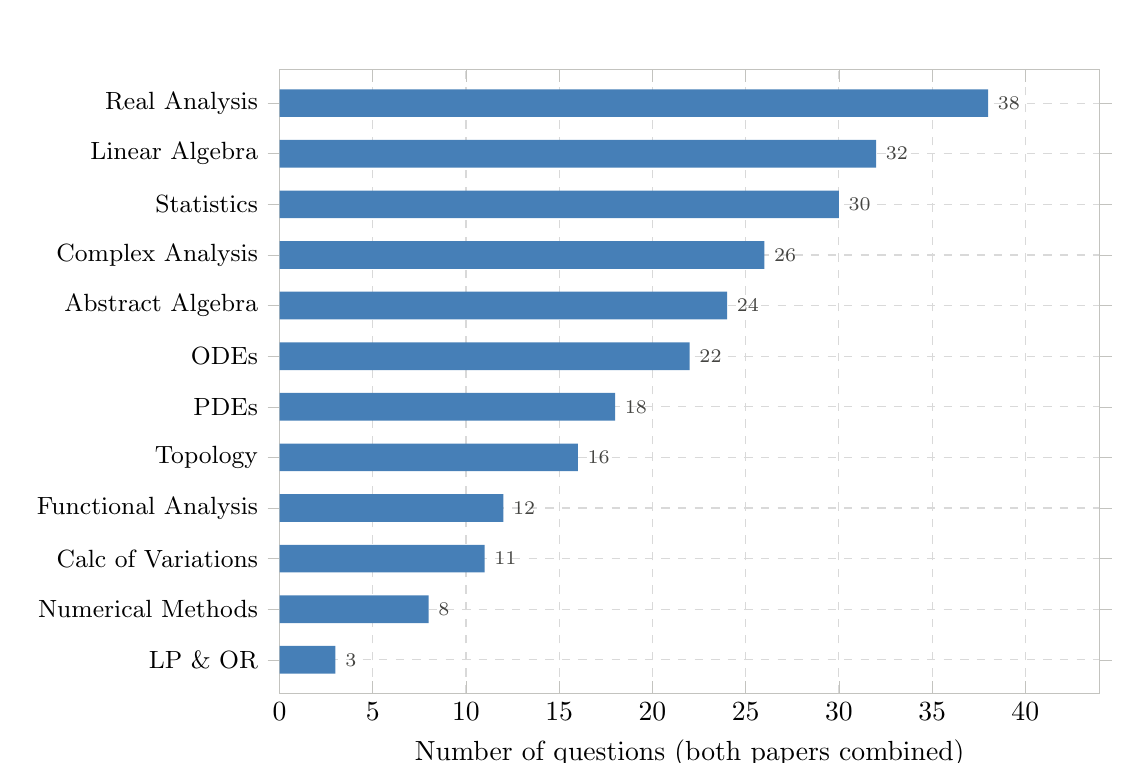
\begin{tikzpicture}
\begin{axis}[
  xbar,
  width=12cm, height=9.5cm,
  bar width=10pt,
  xlabel={Number of questions (both papers combined)},
  symbolic y coords={
    {LP \& OR},
    {Numerical Methods},
    {Calc of Variations},
    {Functional Analysis},
    {Topology},
    {PDEs},
    {ODEs},
    {Abstract Algebra},
    {Complex Analysis},
    {Statistics},
    {Linear Algebra},
    {Real Analysis}
  },
  ytick=data,
  yticklabel style={font=\small},
  nodes near coords,
  nodes near coords align={horizontal},
  every node near coord/.style={font=\scriptsize, color=graydark},
  xmin=0, xmax=44,
  axis line style={color=grayprimary!50},
  tick style={color=grayprimary!50},
  grid=major,
  grid style={color=black!15, dashed},
  enlarge y limits=0.06,
]
\addplot[fill=blueprimary!80, draw=none] coordinates {
  (3,{LP \& OR})
  (8,{Numerical Methods})
  (11,{Calc of Variations})
  (12,{Functional Analysis})
  (16,{Topology})
  (18,{PDEs})
  (22,{ODEs})
  (24,{Abstract Algebra})
  (26,{Complex Analysis})
  (30,{Statistics})
  (32,{Linear Algebra})
  (38,{Real Analysis})
};
\end{axis}
\end{tikzpicture}
\end{center}

\subsection{Part A — General Aptitude (20 questions per paper)}

\begin{center}
\renewcommand{\arraystretch}{1.3}
\begin{tabular}{@{}p{7cm}cc@{}}
\toprule
\rowcolor{bluelight}
\textbf{Sub-topic} & \textbf{Dec 2025} & \textbf{Jun 2025} \\
\midrule
Mathematical reasoning, arithmetic \& ratio problems & 4 & 4 \\
Number theory, sequences, combinatorics & 3 & 3 \\
Logical reasoning (statements, blood relations, coding) & 3 & 3 \\
Data interpretation (pie charts, bar graphs) & 3 & 3 \\
Geometry, distance, area, volume & 2 & 2 \\
Probability \& basic statistics & 2 & 2 \\
Science-based / environmental reasoning & 2 & 2 \\
Current affairs framed as reasoning & 1 & 1 \\
\midrule
\textbf{Total} & \textbf{20} & \textbf{20} \\
\bottomrule
\end{tabular}
\end{center}

\newpage

%% ============================================================
\section{Priority Topic Deep-Dives}
%% ============================================================

\begin{alertred}[Key Insight]
\small Master Tiers 1 and 2 (six topics) and you cover approximately \textbf{75\%} of all Part B and Part C marks. The sub-topics below are exactly what appeared across both 2025 papers.
\end{alertred}

\subsection{Tier 1 — Master First (Highest ROI)}

%% ---- Real Analysis ----
\begin{prioritybox}[1.\quad Real Analysis \hfill\badgered{38 Qs across both papers $\approx$19\% of B+C}]{redprimary}

\textbf{Why it dominates:} Single most tested subject. Questions are deeply conceptual — never purely computational. Appears in every part of every paper.

\medskip
\textbf{Sub-topics to master:}
\begin{itemize}[leftmargin=1.5em, itemsep=2pt]
  \item Sequences and series: convergence tests (ratio, root, comparison), Cauchy sequences, $\limsup$/$\liminf$, rearrangements
  \item Uniform continuity and the composition of uniformly continuous functions
  \item Pointwise vs.\ uniform convergence of sequences of functions; Weierstrass M-test
  \item Riemann integration: Riemann integrable functions, improper integrals on $[0,\infty)$
  \item Monotone functions: one-sided limits always exist; surjective $\Rightarrow$ continuous
  \item Metric space topology: compactness, completeness, distance function $d(x,A)$ (Lipschitz)
  \item Countability arguments: decimal expansions, Cantor-type sets, image under continuous injections
  \item Bounded below / above sets; $\inf A$, $\sup A$ computations for tricky sets
\end{itemize}

\medskip
\textbf{Exact questions from both papers (appear in Part C):}\\
\small Q66 (decimal expansion convergence), Q67 (Riemann integrable on $[0,\infty)$), Q86 (uniform convergence on sub-intervals), Q87 (metric space $d(x,A)$ properties), Q88 (bounded-below set), Q89 (integral function), Q90 (CDF / monotone function), Q92 (fn sequences in $C[0,1]$), Q96 (monotone fn one-sided limits) --- \textit{identical in Dec \& Jun 2025.}
\end{prioritybox}

\vspace{8pt}

%% ---- Linear Algebra ----
\begin{prioritybox}[2.\quad Linear Algebra \hfill\badgepurple{32 Qs across both papers $\approx$16\% of B+C}]{purpleprimary}

\textbf{Why it matters:} Every paper has 4 Part B and 6 Part C Linear Algebra questions. Eigenvalue theory and structural results (projections, quadratic forms) recur without fail.

\medskip
\textbf{Sub-topics to master:}
\begin{itemize}[leftmargin=1.5em, itemsep=2pt]
  \item Eigenvalues, trace, determinant, characteristic polynomial; Newton's power-sum identities
  \item Cayley-Hamilton theorem; minimal polynomial
  \item Diagonalisability over $\mathbb{R}$ and $\mathbb{C}$; Jordan normal form (when does $T^2$ diag.\ $\Rightarrow$ $T$ diag.?)
  \item Inner product spaces: orthonormality, Gram-Schmidt, orthogonal complements
  \item Projections: $T^2=T$ (idempotent), $A^2=I$ operators and their commutant/anticommutant
  \item Quadratic forms: positive definite, signature, Sylvester's law
  \item Rank-nullity; dimension of quotient spaces ($X/\ker\phi$)
  \item Matrices over finite fields $\mathbb{F}_q$: counting matrices of given rank
  \item Invariant subspaces in complex vector spaces; existence of eigenvalues over $\mathbb{C}$
\end{itemize}

\medskip
\textbf{Recurring exact questions:}\\
\small Q74 ($A^2=I$, $\mathrm{Tr}(A)=0$), Q76 ($M_n(\mathbb{C})$ with rank-$k$ inner product), Q78 (spanning set, dimension 4 or 5), Q99 (integer matrix eigenvalues, minimal poly), Q103 ($T^2$ diagonalisable $\Rightarrow$ $T$?), Q107 (4-dim complex VS), Q109 ($T^2=T$ projection), Q113 (sufficient \& ancillary statistics) --- \textit{identical in both papers.}
\end{prioritybox}

\vspace{8pt}

%% ---- Statistics ----
\begin{prioritybox}[3.\quad Statistics \& Probability \hfill\badgeblue{30 Qs across both papers $\approx$15\% of B+C}]{blueprimary}

\textbf{Why it matters:} Highest variety of sub-topics. Also most scoring if you specialise — each sub-topic is self-contained and testable independently.

\medskip
\textbf{Sub-topics to master:}
\begin{itemize}[leftmargin=1.5em, itemsep=2pt]
  \item \textit{Estimation:} MLE (discrete/continuous), UMVUE, sufficient statistics (Factorisation), ancillary statistics, Cramér-Rao bound
  \item \textit{Hypothesis testing:} Neyman-Pearson (UMP tests), LRT, sign test, $p$-values, confidence intervals
  \item \textit{Bayesian:} Beta-Binomial conjugate, posterior mean/variance with improper priors
  \item \textit{Distributions:} Exponential, Gamma, Uniform (MOM/MLE), Binomial, Normal (folded, conditional), Poisson, MGF-based identification
  \item \textit{Multivariate:} $N_p(\mu,\Sigma)$, Wishart distribution, $E(S^{-1})$, partial correlation, multiple correlation
  \item \textit{Markov chains:} Recurrence, transience, positive recurrence, stationary distribution, mean recurrence time
  \item \textit{Regression:} Multiple linear regression, $R^2$, Adjusted $R^2$, $F$-test, BLUE (Gauss-Markov), BLUEs uncorrelated
  \item \textit{Sampling:} SRSWR vs.\ SRSWOR, stratified sampling, unbiased estimators
  \item \textit{Queuing:} $M/M/c$ systems, steady-state probabilities $p_0, p_n$
  \item \textit{Non-parametric:} Sign test, order statistics confidence intervals, survival analysis / hazard rates
  \item \textit{Probability:} CLT, WLLN, convergence in distribution, sequences of i.i.d.\ r.v.'s
\end{itemize}
\end{prioritybox}

\subsection{Tier 2 — High Priority (Do Not Skip)}

\begin{prioritybox}[4.\quad Complex Analysis \hfill\badgeamber{26 Qs $\approx$13\%}]{amberprimary}
\textbf{Sub-topics:}
\begin{itemize}[leftmargin=1.5em, itemsep=2pt]
  \item Holomorphic functions, Cauchy-Riemann equations, analytic continuation
  \item Cauchy's integral theorem and formula; residue theorem (simple/higher-order poles)
  \item Contour integrals on specific paths $\gamma_R(t)=Re^{2\pi it}$; computation of $\int_\gamma \tan z\,dz$ etc.
  \item Singularities: poles (order), essential singularities, removable singularities; Laurent series
  \item Entire functions: Liouville, Picard; growth conditions; image constraints (e.g.\ $f(\mathbb{C})\subset\{y=x+1\}$)
  \item M\"{o}bius (fractional linear) transformations; image of intervals/circles
  \item Schwarz-Pick lemma: $f:\mathbb{D}\to\mathbb{D}$ holomorphic, $|f'(a)|\le \frac{1-|f(a)|^2}{1-|a|^2}$
  \item Function $g(z)=f(z)-\tfrac{1}{z}$: pole at 0, no zeros on unit circle, $\max|g|\ge 1$
  \item Series of holomorphic functions $f_n(z)=\sum_{k=1}^n h(z^k)$; convergence on $\{|z|>1\}$
\end{itemize}
\end{prioritybox}

\vspace{6pt}

\begin{prioritybox}[5.\quad Abstract Algebra \hfill\badgeamber{24 Qs $\approx$12\%}]{amberprimary}
\textbf{Sub-topics:}
\begin{itemize}[leftmargin=1.5em, itemsep=2pt]
  \item Group theory: subgroup counting $S(G)$, Sylow theorems, groups of order 8 / 16 / $p^n$
  \item Permutation groups $S_n$; Burnside's lemma; conjugacy classes
  \item Galois theory: irreducible polynomial of prime degree $p$ with exactly 2 non-real roots $\Rightarrow$ $G=S_p$
  \item Irreducibility tests: Eisenstein, reduction mod $p$; factorisation in $\mathbb{Z}[x]$ and $\mathbb{Q}[x]$
  \item Ring theory: maximal ideals, prime ideals, PIDs, UFDs, Euclidean domains; rings with divisibility property
  \item Number theory: Wilson's theorem, Fermat's little theorem, $p\mid(1234)^{p-1}-1$
  \item Homeomorphisms of finite topological spaces (tied to group counting)
  \item Non-abelian groups: $f(a,b)=ab$ not a homomorphism; normal subgroup count
\end{itemize}
\end{prioritybox}

\vspace{6pt}

\begin{prioritybox}[6.\quad Ordinary Differential Equations \hfill\badgeamber{22 Qs $\approx$11\%}]{amberprimary}
\textbf{Sub-topics:}
\begin{itemize}[leftmargin=1.5em, itemsep=2pt]
  \item IVP existence and uniqueness (Picard-Lindelöf); solutions that are not unique (e.g.\ $y'=f(y)$ with $f$ not Lipschitz)
  \item Taylor series solutions about regular and regular singular points (Frobenius method)
  \item Wronskian: $W(y_1,y_2)$ constant if $p=0$ in $y''+p(x)y'+q(x)y=0$
  \item Sturm-Liouville problems: eigenvalue sequences $\lambda_n$, $\sum 1/\lambda_n$ via Parseval / series identities
  \item Reduction of order: one solution known, find general solution
  \item Integral equations: Volterra $y(x)=f(x)+\int_0^x K(x,t)y(t)dt$; Fredholm $y=f+\lambda\int_{-1}^1 K(x,t)y(t)dt$; resolvent kernel
  \item Oscillation theory: Sturm comparison; zeros of solutions; non-trivial solutions with infinitely many zeros in bounded interval (only if $r(x)$ oscillates)
\end{itemize}
\end{prioritybox}

\subsection{Tier 3 — Selective Mastery (Pick Your Best)}

\begin{center}
\renewcommand{\arraystretch}{1.35}
\begin{tabular}{@{}p{3.2cm}p{9.5cm}c@{}}
\toprule
\rowcolor{bluelight}
\textbf{Topic} & \textbf{Key sub-topics to cover} & \textbf{Qs} \\
\midrule
\textbf{PDEs} & d'Alembert (wave), heat equation with Neumann/Dirichlet BCs, Laplace maximum principle, BVP on disk ($u=e^{x+y}$ on $\partial\Omega$), method of characteristics for first-order PDEs, energy methods for $u_{tt}-u_{xx}+u_t=0$ & 18 \\
\addlinespace
\textbf{Topology} & Product topology (Tychonoff = compact), Hausdorff separation, normality, finite-complement topology (not regular), homeomorphisms of finite spaces, Euclidean topology normality & 16 \\
\addlinespace
\textbf{Functional Analysis} & Hilbert spaces $\ell^2$; set $H=\{(a_n):|a_n|\le 1/n\}$ — bounded, convex, not a subspace, no ONB; compact sets in $C[0,1]$ (Arzelà-Ascoli); operators on Hilbert space & 12 \\
\addlinespace
\textbf{Calc of Variations} & Euler-Lagrange equation; isoperimetric problems ($\int y^2\,dx=1/7$ constraint); transversality conditions; canonical transformations (generating functions, Hamiltonian mechanics) & 11 \\
\addlinespace
\textbf{Numerical Methods} & Newton-Raphson: order of convergence $p$ and asymptotic error constant; Gauss-Seidel convergence (spectral radius of iteration matrix); Lagrange interpolation polynomial; cubic splines continuity conditions & 8 \\
\addlinespace
\textbf{LP \& OR} & Simplex method, optimal feasible solution, $M/M/c$ queuing steady-state probabilities, Linear programming in 2 variables with graphical method & 3--5 \\
\bottomrule
\end{tabular}
\end{center}

\newpage

%% ============================================================
\section{Repeat Patterns — Questions Identical Across Both Papers}
%% ============================================================

\begin{alertred}[Critical Finding]
\small\textbf{18 Part C questions were word-for-word identical} in both December 2025 and June 2025 papers. These represent guaranteed high-value preparation targets. Each carries $+4.75$ marks. Mastering all 18 alone is worth $18\times4.75=\mathbf{85.5}$ marks.
\end{alertred}

\vspace{8pt}

\renewcommand{\arraystretch}{1.35}
\begin{longtable}{@{}p{0.6cm}p{5.5cm}p{8cm}@{}}
\toprule
\rowcolor{bluelight}
\textbf{Q\#} & \textbf{Topic} & \textbf{Exact structure / key idea tested} \\
\midrule
\endfirsthead
\multicolumn{3}{l}{\small\textit{(Continued from previous page)}}\\
\toprule
\rowcolor{bluelight}
\textbf{Q\#} & \textbf{Topic} & \textbf{Exact structure / key idea tested} \\
\midrule
\endhead
\bottomrule
\endlastfoot

Q66 & Decimal expansions (RA) & Strictly increasing $(\beta_n)\nearrow\alpha$ (a finite decimal); $b_{n,2025}=a_{2025}-1$ eventually; digit-by-digit locking \\
\addlinespace
Q67 & Riemann integrable functions (RA) & Four statements about $f:[0,\infty)\to[0,\infty)$; uniformly continuous + convergent integral $\Rightarrow$ $f\to 0$; existence of counterexample with $f\not\to 0$ \\
\addlinespace
Q68 & ODE $y''+r(x)y=0$ (ODE) & $r(x)=x^3\sin(1/x)$; Wronskian = constant; solutions have seq.\ of zeros $\to\infty$; no infinitely-many zeros in bounded interval \\
\addlinespace
Q69 & Product topology (Topology) & $X=\prod_{c>0}[0,c]$; compact (Tychonoff), Hausdorff, connected; \textbf{not} metrizable \\
\addlinespace
Q74 & $A^2=I$, $\mathrm{Tr}(A)=0$ (LA) & Anticommutant $\{B:AB+BA=0\}$ is 8-dim; commutant 8-dim; existence of $B$ with $B^2=I$, $\mathrm{Tr}(B)=0$ \\
\addlinespace
Q75 & $M/M/2$ queue (Statistics) & $\lambda=4$, $\mu=1$, capacity 3; $p_0+p_3=17/29$; $p_3-p_0=15/29$ \\
\addlinespace
Q76 & $M_n(\mathbb{C})$ inner product (LA/FA) & $W_k=\{A:\langle A,B\rangle=0\ \forall\,\mathrm{rank}\text{-}k\, B\}$; $W_1=W_2=W_n=\{0\}$; $W_0\ne\{0\}$ \\
\addlinespace
Q77 & Borrowing / troublesome (Combinatorics) & 6 persons, 12 months, pigeonhole; at least one troublesome in Jan; in any two consecutive months at least one troublesome in one of them \\
\addlinespace
Q78 & Spanning sets (LA) & $\{u,v,w,x,y\}$ spans, $\{u,v,x,y\}$ LI; $\dim V\in\{4,5\}$; $2u-3v+5w=0\Rightarrow\{v,w,x,y\}$ basis \\
\addlinespace
Q79 & Isoperimetric CoV (CoV) & $J(y)=\int_0^1 x^2(y')^2dx$, $y(0)=0$, $y(1)=1$, $\int y^2=1/7$; $y'(1/2)=3/4$, $y'(1/\sqrt{3})=1$ \\
\addlinespace
Q80 & Multivariate Normal / Wishart (Statistics) & $n=20$ from $N_{12}(\mu,\Sigma)$; $E(S^{-1})=\frac{19}{6}\Sigma^{-1}$; $\mathrm{tr}(19\Sigma^{-1}S)\sim\chi^2_{228}$ \\
\addlinespace
Q92 & $f_n=n(1-nx)$ in $C[0,1]$ (FA/RA) & Uniformly bounded; converges pointwise to 0; converges uniformly to 0; set $\{f_n\}$ \textbf{is} compact in $C[0,1]$ \\
\addlinespace
Q93 & $g(z)=f(z)-1/z$ (CA) & $f$ entire; $g$ has pole at 0; no zeros with $|\alpha|=1$; finitely many zeros; $\max_{|z|=1}|g|\ge 1$ \\
\addlinespace
Q94 & $\ell^2$ set $H=\{(a_n):|a_n|\le 1/n\}$ (FA) & Bounded; convex; \textbf{not} a subspace; contains \textbf{no} ONB of $\ell^2$ \\
\addlinespace
Q108 & Galois group $=S_p$ (Algebra) & Irreducible $f\in\mathbb{Q}[x]$ of prime deg.\ $p$, exactly 2 non-real roots; $(12)\in G$; $p$-cycle $\in G$; $G=S_p$ \\
\addlinespace
Q109 & $T^2=T$ projection (LA) & $W=\mathrm{span}\{I,T^n\}$; $\dim W=2$; idempotents in $W$; $U^2=U$, $(T-U)^2=T-U\Rightarrow(TU)^2=TU$ \\
\addlinespace
Q110 & Non-abelian group (Algebra) & $f(a,b)=ab$ not a homomorphism; every divisor has subgroup $\Rightarrow\ge 3$ normal subgroups \\
\addlinespace
Q120 & $f(z)=\sin^2z+\cos^2|z|$ (CA) & Not real-valued; not entire; not identically 1; finitely many zeros on imaginary axis \\
\bottomrule
\end{longtable}

\subsection{Recurring Sub-topic Patterns (Across Multiple Questions)}

\begin{center}
\renewcommand{\arraystretch}{1.25}
\begin{tabular}{@{}p{3.5cm}p{9.5cm}@{}}
\toprule
\rowcolor{bluelight}
\textbf{Pattern} & \textbf{What to study} \\
\midrule
Trace-eigenvalue identities & Newton's identities; $\mathrm{tr}(A)=\sum\lambda_i$, $\mathrm{tr}(A^2)=\sum\lambda_i^2$; char poly from trace data \\
Uniform vs.\ pointwise & Weierstrass M-test; sequences $f_n$ on $[0,1]$; Dini's theorem \\
Contour integrals on $\gamma_R$ & Residue theorem at $z=\pi/2$ ($\tan z$), $z=0$ ($z\sin z$); winding numbers \\
Beta-Binomial Bayesian & Posterior mean = $\frac{X+\alpha}{n+\alpha+\beta}$; posterior $\gtrless$ prior mean iff $X/n\gtrless\alpha/(\alpha+\beta)$ \\
Markov chain classification & States: recurrent / transient / ergodic; stationary $\pi P=\pi$; mean return time \\
Fredholm integral equations & Degenerate kernels; eigenvalues $\lambda$ of $K$; resolvent $R(x,t;\lambda)$ \\
Möbius image of real line & $f(z)=(z-i)/(z+i)$; images of intervals and lines as arcs / semicircles \\
Gauss-Seidel convergence & Spectral radius of $T_{GS}=-(D+L)^{-1}U$ must be $<1$ \\
Newton-Raphson order & $p=2$ for simple zero; $p=1$ for multiple / inflection ($\sin x=1$ at $\pi/2$) \\
Cubic splines & $C^2$ continuity conditions; $2a+b+2c=$ specific value from both papers \\
\bottomrule
\end{tabular}
\end{center}

\newpage

%% ============================================================
\section{Part-wise Question Split Tables}
%% ============================================================

\subsection{Part B — MCQ (40 questions per paper, attempt 25)}

\begin{center}
\renewcommand{\arraystretch}{1.35}
\begin{tabular}{@{}lcccc@{}}
\toprule
\rowcolor{bluelight}
\textbf{Topic} & \textbf{Dec 2025} & \textbf{Jun 2025} & \textbf{Expected Range} & \textbf{Recommend attempt?} \\
\midrule
Statistics \& Probability & 5 & 5 & 5 & \badgegreen{Yes — all 5} \\
Real Analysis & 4 & 5 & 4--5 & \badgegreen{Yes — 4--5} \\
Linear Algebra & 4 & 4 & 4 & \badgegreen{Yes — all 4} \\
Complex Analysis & 4 & 4 & 4 & \badgegreen{Yes — 3--4} \\
Abstract Algebra & 4 & 4 & 4 & \badgegreen{Yes — 3--4} \\
ODEs & 3 & 3 & 3 & \badgeamber{Yes — 2--3} \\
PDEs & 3 & 2 & 2--3 & \badgeamber{Yes — 2} \\
Topology & 2 & 2 & 2 & \badgeamber{Selective} \\
Numerical Methods & 2 & 2 & 2 & \badgeamber{Yes — if prepared} \\
Calculus of Variations & 2 & 2 & 2 & \badgeamber{Yes — if prepared} \\
Functional Analysis & 1 & 1 & 1 & \badgegray{If fast to solve} \\
Linear Programming & 1 & 1 & 1 & \badgegreen{Yes — easy marks} \\
\midrule
\textbf{Total Part B} & \textbf{35--40} & \textbf{35--40} & \textbf{40} & \textit{Attempt: 25} \\
\bottomrule
\end{tabular}
\end{center}

\subsection{Part C — MSQ (60 questions per paper, attempt 20)}

\begin{center}
\renewcommand{\arraystretch}{1.35}
\begin{tabular}{@{}lcccc@{}}
\toprule
\rowcolor{bluelight}
\textbf{Topic} & \textbf{Dec 2025} & \textbf{Jun 2025} & \textbf{Expected Range} & \textbf{Recommend attempt?} \\
\midrule
Real Analysis & 9 & 8 & 8--9 & \badgegreen{Select 4--5} \\
Statistics \& Probability & 8 & 8 & 8 & \badgegreen{Select 4--5} \\
Linear Algebra & 6 & 6 & 6 & \badgegreen{Select 3--4} \\
Complex Analysis & 6 & 5 & 5--6 & \badgegreen{Select 2--3} \\
Abstract Algebra & 5 & 5 & 5 & \badgegreen{Select 2--3} \\
ODEs & 4 & 4 & 4 & \badgeamber{Select 1--2} \\
PDEs & 4 & 4 & 4 & \badgeamber{Select 1--2} \\
Topology & 4 & 4 & 4 & \badgeamber{Select 1--2} \\
Functional Analysis & 3 & 3 & 3 & \badgeamber{Select 1} \\
Calculus of Variations & 3 & 3 & 3 & \badgeamber{Select 1} \\
Numerical Methods & 2 & 2 & 2 & \badgegray{Selective} \\
Classical Mechanics & 2 & 2 & 2 & \badgegray{Selective} \\
Combinatorics / Logic & 2 & 1 & 1--2 & \badgegray{Selective} \\
\midrule
\textbf{Total Part C} & \textbf{58--60} & \textbf{55--60} & \textbf{60} & \textit{Attempt: 20} \\
\bottomrule
\end{tabular}
\end{center}

\newpage

%% ============================================================
\section{12-Week Preparation Schedule}
%% ============================================================

\begin{alertblue}[Plan Overview]
\small Four phases: \textbf{Weeks 1--4} build the top-3 topics deep. \textbf{Weeks 5--8} cover the next three topics. \textbf{Weeks 9--10} tackle remaining topics. \textbf{Weeks 11--12} are full timed mock tests with gap analysis. Adjust based on existing knowledge.
\end{alertblue}

\vspace{10pt}

\subsection*{Phase 1 — Foundation (Weeks 1--4): Real Analysis + Linear Algebra}

\weekblock{1}{Real Analysis I — Sequences, Series, Continuity}{
Convergence tests (ratio, root, comparison), Cauchy sequences, $\limsup/\liminf$, Abel/Dirichlet summability, uniform continuity definition and properties, Weierstrass M-test. \textit{Solve:} Dec Q33, Q36, Q39, Q47, Q49; Jun Q24, Q25, Q26, Q56. \textbf{Target:} 10+ hours.
}

\weekblock{2}{Real Analysis II — Metric Spaces, Integration, Monotone Functions}{
Metric space compactness, $d(x,A)$ Lipschitz continuity, Riemann integrable functions on $[0,\infty)$, monotone function one-sided limits, $\sup$/$\inf$ of tricky sets, countability. \textit{Solve all 9 identical Part C questions}: Q66--Q68, Q86--Q90, Q92, Q96. \textbf{Target:} 10+ hours.
}

\weekblock{3}{Linear Algebra I — Eigenvalues, Trace, Diagonalisability}{
Newton's power-sum identities, char poly from trace data, Cayley-Hamilton, diagonalisability criteria, minimal polynomial, Jordan normal form basics. \textit{Solve:} Dec Q23, Q25, Q45, Q53; Jun Q27, Q28, Q29, Q30. \textbf{Target:} 10 hours.
}

\weekblock{4}{Linear Algebra II — Projections, Inner Products, Quadratic Forms, Finite Fields}{
$T^2=T$ and $A^2=I$ structures, $M_n(\mathbb{C})$ inner product, $W_k$ spaces, vector space spanning dimension argument, quadratic form signature, matrices over $\mathbb{F}_q$. \textit{Solve identical C questions:} Q74, Q76, Q78, Q99, Q103, Q107, Q109. \textbf{Target:} 10 hours.
}

\subsection*{Phase 2 — Core Expansion (Weeks 5--8): Algebra + Complex Analysis + Statistics}

\weekblock{5}{Complex Analysis — Holomorphic Functions, Singularities, Contour Integrals}{
Cauchy's theorem, residue theorem, classification of singularities, Taylor/Laurent series, entire functions (Liouville, Picard), contour integrals on $\gamma_R(t)=Re^{2\pi it}$. \textit{Solve:} Dec Q28, Q41, Q42, Q44; identical C Qs Q93, Q120. Also Schwarz-Pick (Q101). \textbf{Target:} 10 hours.
}

\weekblock{6}{Abstract Algebra — Groups, Rings, Galois Theory}{
Sylow theorems, groups of order 8, Galois group $=S_p$ (irreducible poly, 2 non-real roots), Eisenstein criterion, maximal/prime ideals, rings with divisibility, Wilson/Fermat. \textit{Solve:} Dec Q22, Q30, Q60, Q62, Q65; identical C Qs Q108, Q110. \textbf{Target:} 10 hours.
}

\weekblock{7}{Statistics I — Estimation, Testing, Bayesian}{
MLE, sufficient statistics (Factorisation theorem), ancillary statistics, UMP tests (Neyman-Pearson), LRT, Beta-Binomial conjugate, confidence intervals for various distributions. \textit{Solve:} Dec Q21, Q51, Q54, Q55, Q57; Jun Q53, Q54, Q55, Q56. \textbf{Target:} 12 hours.
}

\weekblock{8}{Statistics II — Multivariate, Markov Chains, Regression, Sampling}{
Wishart distribution, $E(S^{-1})$, partial correlation, Markov chain classification (recurrence/transience), multiple regression $R^2$/$F$-test, SRSWOR/stratified sampling, $M/M/c$ queuing, sign test. \textit{Solve identical C Qs:} Q75, Q77, Q80, Q97, Q98. \textbf{Target:} 12 hours.
}

\subsection*{Phase 3 — Secondary Topics (Weeks 9--10)}

\weekblock{9}{ODEs + PDEs + Integral Equations}{
Frobenius method, Sturm-Liouville $\sum 1/\lambda_n$, Wronskian constancy, Fredholm/Volterra integral equations, resolvent kernel; PDE: d'Alembert, heat equation with BCs, Laplace (maximum principle), method of characteristics, energy method. \textit{Solve identical Q:} Q68, Q72, Q79, Q81, Q84, Q116, Q118. \textbf{Target:} 12 hours.
}

\weekblock{10}{Topology + Functional Analysis + CoV + Numerical Methods}{
Product topology Tychonoff, normality, $\ell^2$ Hilbert space (set $H$), compact sets in $C[0,1]$, Euler-Lagrange with isoperimetric constraints, Newton-Raphson order-2 convergence, Gauss-Seidel spectral radius, Lagrange interpolation, cubic splines. \textit{Solve identical Qs:} Q69, Q71, Q79, Q82, Q92, Q94. \textbf{Target:} 10 hours.
}

\subsection*{Phase 4 — Mock Tests \& Final Revision (Weeks 11--12)}

\weekblock{11}{Full Mock — December 2025 Paper (timed: 180 minutes)}{
Part A: 20 min. Part B: 60 min. Part C: 100 min. Record which questions you got wrong and why. Categorise errors: conceptual gap / calculation error / misread / time pressure. Identify weakest 2--3 sub-topics. \textbf{Target:} 1 full test + 4 hrs gap analysis.
}

\weekblock{12}{Full Mock — June 2025 Paper + Targeted Revision}{
Attempt June 2025 under strict timed conditions. Revise weakest sub-topics from Week 11 analysis. Final day: revise all 18 identical Part C questions (maximum ROI per hour). Prepare a one-page \textit{cheat sheet} of key theorems for last-day review. \textbf{Target:} 1 full test + 4 hrs targeted revision.
}

\newpage

%% ============================================================
\section{Exam Day Strategy}
%% ============================================================

\subsection{Part A — General Aptitude (20 minutes recommended)}

\begin{itemize}[leftmargin=1.5em, itemsep=4pt]
  \item \textbf{Attempt only 15 of 20.} Score if all 15 correct: $15\times2=30$. If you attempt 15 correct + 5 wrong: $30-2.5=27.5$. Never guess.
  \item \textbf{Recommended order:} Arithmetic/ratio problems first (fastest) $\to$ Logical reasoning $\to$ Data interpretation $\to$ Geometry/science (slowest).
  \item \textbf{Time rule:} $\le 75$ seconds per question. If stuck after 45 seconds, skip and return.
  \item Both 2025 papers had 8 arithmetic + 6 logic questions — these are the most predictable category.
\end{itemize}

\subsection{Part B — MCQ (60 minutes recommended)}

\begin{itemize}[leftmargin=1.5em, itemsep=4pt]
  \item \textbf{Scan all 40 questions first (5 minutes).} Mark each: \checkmark\,(very confident), ?\,(partial), $\times$\,(skip).
  \item Solve all \checkmark\,first, then revisit ?\,with remaining time. Never attempt $\times$ unless surplus time and near-certainty.
  \item \textbf{Attempt exactly 25 — never more.} Penalty is $-0.75$ or $-1$ per wrong answer.
  \item Recommended topic-wise count: Statistics (5) + Real Analysis (4--5) + Linear Algebra (4) + Complex Analysis (3--4) + Abstract Algebra (3--4) + ODEs/PDEs (3) + LP/Numerical (2) = 24--26 total. Choose your strongest.
  \item $\approx 2.4$ minutes per question. Statistics and LP tend to be fastest; Topology and Functional Analysis slowest.
\end{itemize}

\subsection{Part C — MSQ (100 minutes recommended)}

\begin{alertamber}[The 90\% Confidence Rule]
\small In Part C, only select an option if you are \textbf{at least 90\% confident} it is correct. If you know options 1 and 3 are correct but are unsure about option 2 --- select only 1 and 3. The $-1.25$ penalty for any wrong option destroys both the penalty cost and the full $+4.75$ credit simultaneously.
\end{alertamber}

\begin{itemize}[leftmargin=1.5em, itemsep=4pt]
  \item \textbf{Attempt exactly 20 questions.} Target: 18--19 fully correct $=$ 85.5--90.25 marks from Part C alone.
  \item \textbf{Prioritise the 18 identical questions} (Q66--Q120 range). You already know their exact structure and correct answers from preparation. These are free marks.
  \item \textbf{Recommended selection order:} Real Analysis (pick 4) $\to$ Statistics (pick 4) $\to$ Linear Algebra (pick 3) $\to$ Complex Analysis (pick 3) $\to$ Abstract Algebra (pick 2) $\to$ ODEs/PDEs/Topology (pick remaining 4).
  \item For each question: identify the options you are \textit{certain} are correct and the options you are \textit{certain} are wrong. Select only the former. Leave unresolved options unselected.
  \item \textbf{Time management:} Read every option carefully. An average of 5 minutes per question is appropriate — some will take 2 minutes, some 8 minutes.
\end{itemize}

\subsection{Common Traps to Avoid}

\begin{center}
\renewcommand{\arraystretch}{1.3}
\begin{tabular}{@{}p{5cm}p{9cm}@{}}
\toprule
\rowcolor{redlight}
\textbf{Trap} & \textbf{How to avoid it} \\
\midrule
Selecting a ``seems right'' MSQ option & Apply the 90\% rule. If you have any doubt, leave it unselected. \\
Attempting 26+ questions in Part B & The 26th attempt on a wrong answer costs you 1 mark net. Stop at 25. \\
Confusing pointwise vs.\ uniform convergence & Uniform: $\sup_x|f_n(x)-f(x)|\to 0$. Pointwise: only fix $x$. Completely different! \\
Missing ``NECESSARILY TRUE'' qualifier & A statement must hold for \textit{all} instances in the given class, not just one example. \\
FALSE vs.\ NOT FALSE questions & Jun Q32, Q33, Q38 ask which statement is \textbf{FALSE}. Invert your reasoning. \\
Misreading Möbius image & Always compute what happens to 3 points on the domain. Use the circle/line preservation property. \\
Part C: selecting all 4 options reflexively & When you're 90\% sure about 3 options and 50/50 on the 4th --- skip the 4th. \\
Skipping Part C entirely for a topic & Even one fully-correct answer in a weak topic (4.75 marks) beats 2 wrong Part B attempts ($-2$ marks). \\
\bottomrule
\end{tabular}
\end{center}

\newpage

%% ============================================================
\section{Recommended Study Resources}
%% ============================================================

\begin{center}
\renewcommand{\arraystretch}{1.35}
\begin{tabular}{@{}p{3.5cm}p{5cm}p{5.5cm}@{}}
\toprule
\rowcolor{bluelight}
\textbf{Topic} & \textbf{Primary Reference} & \textbf{Supplementary} \\
\midrule
Real Analysis & W.\ Rudin, \textit{Principles of Mathematical Analysis} & Apostol, \textit{Mathematical Analysis} \\
Linear Algebra & S.\ Axler, \textit{Linear Algebra Done Right} & Hoffman \& Kunze, \textit{Linear Algebra} \\
Abstract Algebra & Dummit \& Foote, \textit{Abstract Algebra} & Herstein, \textit{Topics in Algebra} \\
Complex Analysis & L.\ Ahlfors, \textit{Complex Analysis} & Conway, \textit{Functions of One Complex Variable} \\
Topology & J.R.\ Munkres, \textit{Topology} & Simmons, \textit{Introduction to Topology} \\
ODEs & Coddington \& Levinson, \textit{ODE Theory} & Birkhoff \& Rota, \textit{Ordinary Differential Equations} \\
PDEs & L.C.\ Evans, \textit{Partial Differential Equations} & Strauss, \textit{PDEs: An Introduction} \\
Functional Analysis & E.\ Kreyszig, \textit{Introductory FA} & Simmons, \textit{Introduction to FA} \\
Statistics & Hogg, McKean \& Craig, \textit{Mathematical Statistics} & Casella \& Berger, \textit{Statistical Inference} \\
Probability & S.M.\ Ross, \textit{Introduction to Probability Models} & Billingsley, \textit{Probability \& Measure} \\
Calculus of Variations & I.M.\ Gelfand \& Fomin & Elsgolts, \textit{Differential Equations \& CoV} \\
Numerical Methods & S.S.\ Sastry, \textit{Introductory Methods of Numerical Analysis} & Burden \& Faires, \textit{Numerical Analysis} \\
\bottomrule
\end{tabular}
\end{center}

\subsection{Practice Material}

\begin{itemize}[leftmargin=1.5em, itemsep=4pt]
  \item \textbf{Past papers (highest priority):} Solve last 10 years of CSIR papers in strict timed conditions. The Dec 2025 and Jun 2025 papers in this document are the most recent and most predictive.
  \item \textbf{Official source:} NTA website (\texttt{csirnet.nta.nic.in}) for official answer keys and previous papers.
  \item \textbf{Topic-specific banks:} NBHM PhD question papers for Real Analysis, Linear Algebra, and Complex Analysis contain questions of comparable depth.
  \item \textbf{CMI/ISI entrance exams:} Excellent supplementary practice for Abstract Algebra and Real Analysis.
\end{itemize}

%% ============================================================
\section{Quick-Reference Summary Sheet}
%% ============================================================

\begin{tcolorbox}[
  enhanced, breakable,
  colback=bluelight!40, colframe=blueprimary,
  boxrule=1pt, arc=6pt,
  title={\textbf{At-a-Glance: What to Study, In What Order}},
  fonttitle=\bfseries\color{white},
  attach boxed title to top left={yshift=-3mm, xshift=6mm},
  boxed title style={colback=blueprimary, arc=4pt}
]
\small
\begin{enumerate}[leftmargin=1.5em, itemsep=3pt]
  \item \textbf{Real Analysis} (Week 1--2): \textit{uniform convergence, metric spaces, Riemann integration, monotone functions, countability}
  \item \textbf{Linear Algebra} (Week 3--4): \textit{char poly, Cayley-Hamilton, $T^2=T$/$A^2=I$, inner products, $W_k$ spaces, $\mathbb{F}_q$ matrices}
  \item \textbf{Complex Analysis} (Week 5): \textit{residue theorem, $g(z)=f(z)-1/z$, Möbius maps, Schwarz-Pick, entire functions}
  \item \textbf{Abstract Algebra} (Week 6): \textit{Galois $G=S_p$, groups of order 8, irreducibility (Eisenstein), maximal ideals}
  \item \textbf{Statistics} (Week 7--8): \textit{MLE, UMP tests, Bayesian (Beta-Binomial), Wishart, Markov chains, $M/M/2$ queue, multiple regression}
  \item \textbf{ODEs + PDEs} (Week 9): \textit{Sturm-Liouville, Frobenius, integral equations, d'Alembert wave, heat BVP, energy method}
  \item \textbf{Topology + FA + CoV + Numerical} (Week 10): \textit{product topology, $\ell^2$, Euler-Lagrange, N-R order 2, Gauss-Seidel}
  \item \textbf{Mock tests} (Week 11--12): \textit{Dec 2025 paper $\to$ gap analysis $\to$ Jun 2025 paper $\to$ final revision of 18 identical Qs}
\end{enumerate}
\tcblower
\small\textbf{Part C non-negotiables (memorise these):}
$M/M/2$ queue ($\lambda=4$, $\mu=1$, cap 3) $\cdot$ Product topology $\prod[0,c]$ (compact, Hausdorff, connected, not metrizable) $\cdot$ $A^2=I$, $\mathrm{Tr}(A)=0$: anticommutant is 8-dim $\cdot$ Galois: irred.\ prime deg., 2 non-real roots $\Rightarrow G=S_p$ $\cdot$ $g(z)=f(z)-1/z$: pole at 0, no zero on $|z|=1$ $\cdot$ $f_n=n(1-nx)$: compact in $C[0,1]$, converges uniformly to 0 $\cdot$ $H=\{(a_n):|a_n|\le 1/n\}\subset\ell^2$: bounded + convex, not a subspace $\cdot$ $f(z)=\sin^2z+\cos^2|z|$: not entire, finitely many zeros on imaginary axis
\end{tcolorbox}

\vspace{10pt}

\begin{alertgreen}[Final Motivation]
\small
The 18 identical questions alone are worth \textbf{85.5 marks out of 200}. The top 6 topics cover \textbf{$\sim$75\% of Part B+C marks}. A focused, topic-prioritised approach with strong Part C discipline is the single most effective strategy for CSIR NET Mathematical Sciences.\\[4pt]
\textit{Good luck!}
\end{alertgreen}

%% ============================================================
\vspace*{\fill}
\begin{center}
\small\color{grayprimary}
Blueprint based on CSIR-UGC NET Mathematical Sciences --- December 2025 (Code 704, Shift 2) \& June 2025 (Code 704, Shift 2)\\
NTA Final Answer Keys used for all 240 questions. Compile with \texttt{pdflatex} (run twice for table of contents).
\end{center}

\end{document}
